% SECTION ====================================================================================
\section{Suchen}
% ============================================================================================
\vspace{-4pt}
\begin{sectionbox}
\subsection{Divide and Conquer}\smallskip
\begin{tabular*}{\columnwidth}{@{\extracolsep\fill}ll@{}}
Gegeben: & Sortiertes Array $A$ mit $n$ Elementen und einen Schlüssel b \\
Gesucht: & Index k mit $A[k]=b$ \\
Lösung: & Zeiger und Halbierung des Arrays\\
\end{tabular*}

\begin{center}
    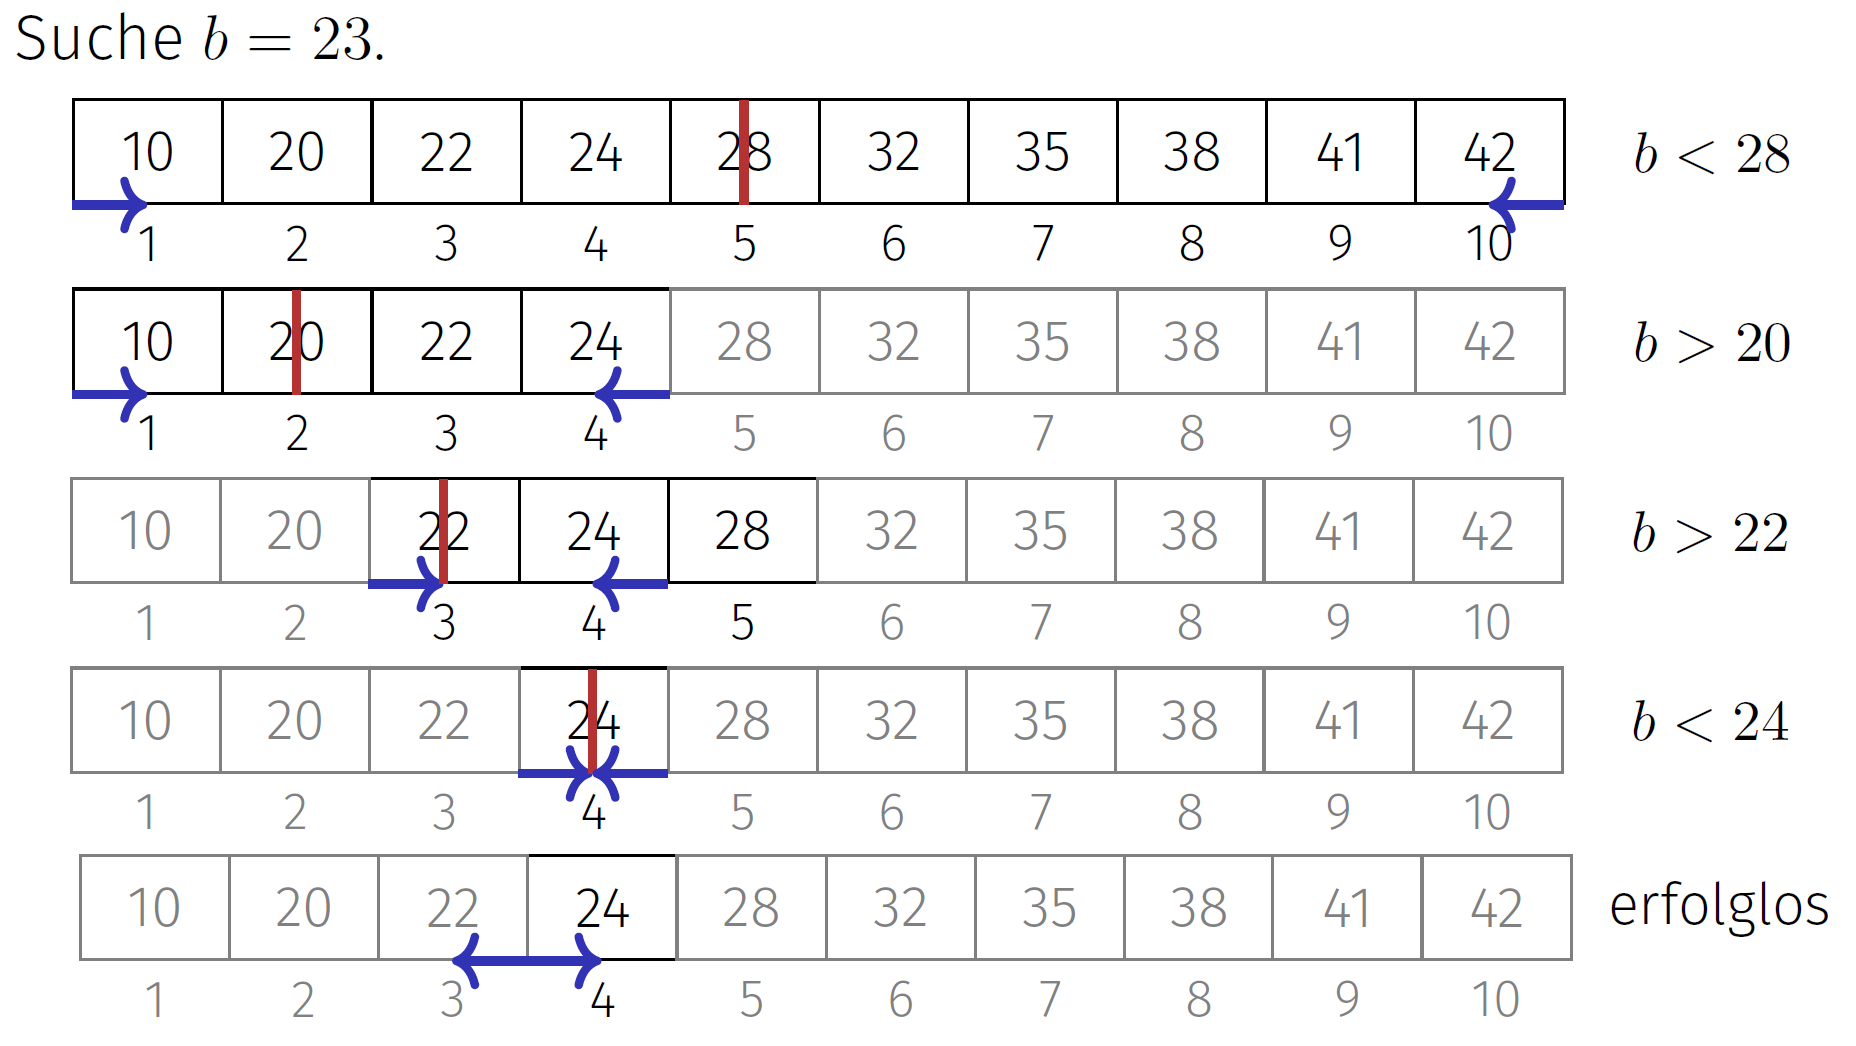
\includegraphics[width = 0.6\columnwidth]{../img/DaQ.png}
\end{center}\par\smallskip
\end{sectionbox}
\vspace{-4pt}
\begin{sectionbox}
\subsection{Binärer Suchalgorithmus: BSearch(A,l,r,b)}\smallskip
\begin{center}
    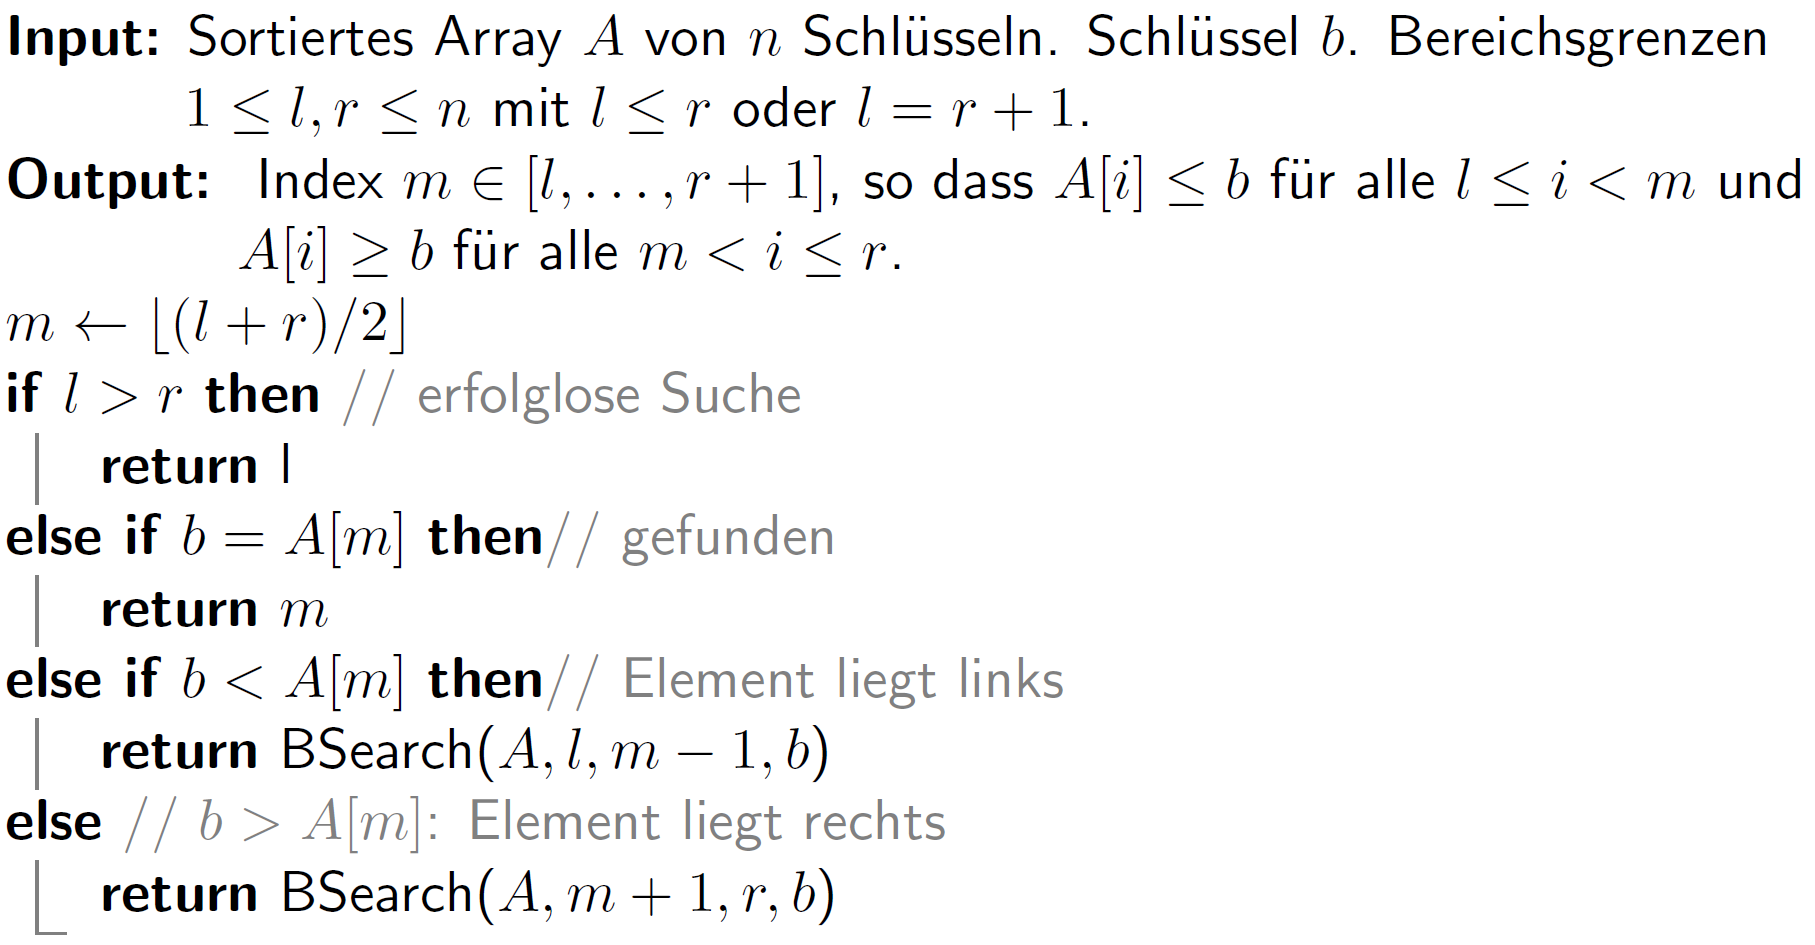
\includegraphics[width = \columnwidth]{../img/BSearch.png}
\end{center}\par\smallskip
\end{sectionbox}